\documentclass[11pt,a4paper]{article}

\usepackage{lmodern}
\usepackage[T1]{fontenc}
\usepackage[utf8]{inputenc}
\usepackage[margin=2.3cm]{geometry}
\usepackage{graphicx}
\usepackage{booktabs}
\usepackage{amsmath}
\usepackage{float}
\usepackage{caption}
\usepackage[table]{xcolor}
\usepackage[hidelinks]{hyperref}

\graphicspath{{prog1_mandelbrot_threads/}{prog2_vecintrin/}}

\setlength{\emergencystretch}{3em}   % let TeX stretch rather than overflow
\setlength{\parskip}{0.5em}
\setlength{\parindent}{0pt}
\captionsetup{font=small}

\newcommand{\ms}[1]{#1\,ms}

% Tables generated by prog1_mandelbrot_threads/make_tables.py directly from
% the CSV files written by measure.sh.
% Generated by make_tables.py from measure.sh output. Do not edit.
\newcommand{\progOneSpeedupViewOne}{%
\begin{tabular}{r rrr rrr rrr}
\toprule
 & \multicolumn{3}{c}{Block} & \multicolumn{3}{c}{Row-cyclic} & \multicolumn{3}{c}{Row-cyclic, \texttt{nice -20}} \\
\cmidrule(lr){2-4}\cmidrule(lr){5-7}\cmidrule(lr){8-10}
Threads & ms & speedup & eff. & ms & speedup & eff. & ms & speedup & eff. \\
\midrule
2 & 243.797 & 1.92 & 0.96 & 244.231 & 1.95 & 0.97 & 237.254 & 1.89 & 0.94 \\
3 & 288.797 & 1.62 & 0.54 & 165.712 & 2.85 & 0.95 & 161.303 & 2.77 & 0.92 \\
4 & 198.410 & 2.36 & 0.59 & 127.960 & 3.64 & 0.91 & 124.252 & 3.61 & 0.90 \\
5 & 194.412 & 2.40 & 0.48 & 107.466 & 4.34 & 0.87 & 106.670 & 4.19 & 0.84 \\
6 & 151.944 & 3.10 & 0.52 & 89.962 & 5.21 & 0.87 & 89.495 & 5.00 & 0.83 \\
7 & 144.400 & 3.25 & 0.46 & 77.278 & 6.05 & 0.86 & 76.944 & 5.82 & 0.83 \\
8 & 124.331 & 3.79 & 0.47 & 86.399 & 5.42 & 0.68 & 67.373 & 6.66 & 0.83 \\
16 & 80.088 & 5.85 & 0.37 & 76.654 & 6.13 & 0.38 & 70.809 & 6.33 & 0.40 \\
\bottomrule
\end{tabular}
}

\newcommand{\progOneSpeedupViewTwo}{%
\begin{tabular}{r rrr rrr rrr}
\toprule
 & \multicolumn{3}{c}{Block} & \multicolumn{3}{c}{Row-cyclic} & \multicolumn{3}{c}{Row-cyclic, \texttt{nice -20}} \\
\cmidrule(lr){2-4}\cmidrule(lr){5-7}\cmidrule(lr){8-10}
Threads & ms & speedup & eff. & ms & speedup & eff. & ms & speedup & eff. \\
\midrule
2 & 166.452 & 1.66 & 0.83 & 142.846 & 1.92 & 0.96 & 140.189 & 1.88 & 0.94 \\
3 & 129.302 & 2.12 & 0.71 & 97.807 & 2.80 & 0.93 & 95.286 & 2.77 & 0.92 \\
4 & 109.890 & 2.51 & 0.63 & 76.322 & 3.61 & 0.90 & 73.332 & 3.59 & 0.90 \\
5 & 98.715 & 2.79 & 0.56 & 64.436 & 4.28 & 0.86 & 63.737 & 4.14 & 0.83 \\
6 & 84.791 & 3.25 & 0.54 & 54.004 & 5.10 & 0.85 & 53.639 & 4.91 & 0.82 \\
7 & 77.708 & 3.52 & 0.50 & 46.516 & 5.94 & 0.85 & 46.201 & 5.71 & 0.82 \\
8 & 69.871 & 3.97 & 0.50 & 49.667 & 5.55 & 0.69 & 40.522 & 6.52 & 0.81 \\
16 & 46.698 & 5.94 & 0.37 & 45.577 & 6.06 & 0.38 & 42.498 & 6.20 & 0.39 \\
\bottomrule
\end{tabular}
}

\newcommand{\progOnePriority}{%
\begin{tabular}{r rrr}
\toprule
Threads & Normal priority & \texttt{nice -20} & Change \\
\midrule
2 & 1.95 & 1.89 & $-3.1\%$ \\
3 & 2.85 & 2.77 & $-2.8\%$ \\
4 & 3.64 & 3.61 & $-0.8\%$ \\
5 & 4.34 & 4.19 & $-3.5\%$ \\
6 & 5.21 & 5.00 & $-4.0\%$ \\
7 & 6.05 & 5.82 & $-3.8\%$ \\
8 & 5.42 & 6.66 & $+22.9\%$ $\star$ \\
16 & 6.13 & 6.33 & $+3.3\%$ \\
\bottomrule
\end{tabular}
}

\newcommand{\progOneBalanceFour}{%
\begin{tabular}{r rr}
\toprule
Thread & Block (ms) & Row-cyclic (ms) \\
\midrule
0 & 50.0 & 129.4 \\
1 & 198.5 & 124.9 \\
2 & 198.9 & 125.2 \\
3 & 47.4 & 126.0 \\
\midrule
slowest & \textbf{198.9} & \textbf{129.4} \\
spread & 4.2$\times$ & 1.0$\times$ \\
\bottomrule
\end{tabular}
}

\newcommand{\progOneBalanceEight}{%
\begin{tabular}{r rr}
\toprule
Thread & Block (ms) & Row-cyclic (ms) \\
\midrule
0 & 9.3 & 67.4 \\
1 & 42.9 & 67.2 \\
2 & 87.3 & 67.4 \\
3 & 122.0 & 88.6 \\
4 & 124.4 & 67.4 \\
5 & 87.5 & 67.2 \\
6 & 43.2 & 67.4 \\
7 & 9.8 & 69.9 \\
\midrule
slowest & \textbf{124.4} & \textbf{88.6} \\
spread & 13.3$\times$ & 1.3$\times$ \\
\bottomrule
\end{tabular}
}


% Generated by plot_prog2.py from measure_prog2.sh output.
\newcommand{\progTwoWidths}{%
\begin{tabular}{r rr rr rr}
\toprule
Width & Vector & Reduction & Utilized & Total & Utilization & Inner-loop \\
 & instructions & vs width 2 & lanes & lanes & (measured) & utilization \\
\midrule
2 & 167\,515 & 1.00$\times$ & 294\,622 & 335\,030 & 87.9\% & 73.2\% \\
4 & 97\,071 & 1.73$\times$ & 321\,252 & 388\,284 & 82.7\% & 60.1\% \\
8 & 52\,877 & 3.17$\times$ & 338\,624 & 423\,016 & 80.0\% & 53.9\% \\
16 & 27\,592 & 6.07$\times$ & 347\,864 & 441\,472 & 78.8\% & 51.0\% \\
\bottomrule
\end{tabular}}

\newcommand{\progTwoDivergence}{%
\begin{tabular}{r rrrr}
\toprule
Width & Loop iterations & Lane capacity & Wasted lanes & Useful \\
\midrule
2 & 30\,628 & 61\,256 & 16\,421 & 73.2\% \\
4 & 18\,642 & 74\,568 & 29\,733 & 60.1\% \\
8 & 10\,406 & 83\,248 & 38\,413 & 53.9\% \\
16 & 5\,491 & 87\,856 & 43\,021 & 51.0\% \\
\bottomrule
\end{tabular}}


\title{\vspace{-1.5cm}\textbf{CS3006 --- Parallel and Distributed Computing}\\[0.3em]
       \large Assignment 2: Performance Analysis on a Multi-Core CPU}
\author{Abdul Muhaimin \\ Roll number: 23L-0775}
\date{\today}

\begin{document}
\maketitle

%======================================================================
\section{Machine Declaration}
%======================================================================

All measurements in this report were taken on the single machine described
below. No result was produced on any other machine.

\begin{table}[H]
\centering
\begin{tabular}{l p{10.3cm}}
\toprule
\textbf{Field} & \textbf{Value} \\
\midrule
CPU model                 & Intel Core i7-7820HQ @ 2.90\,GHz (Kaby Lake, mobile) \\
Physical cores            & 4 \quad ($C = 4$) \\
Hardware threads          & 8 \quad ($T = 8$) \\
SMT / Hyper-Threading     & Present, enabled --- 2 threads per core \\
Base clock                & 2.90\,GHz \\
Maximum turbo clock       & 3.90\,GHz rated; 3.913\,GHz observed single-threaded \\
Widest SIMD unit          & AVX2 --- 256-bit, $W = 8$ single-precision lanes \\
                          & (AVX-512 is \emph{not} present on this part) \\
RAM size and type         & 16\,GB DDR4-2667 (\texttt{MemTotal} 16\,249\,212\,kB) \\
                          & \textbf{Single-channel}: one 16\,GB DIMM in Channel~A;
                            Channel~B empty \\
                          & Theoretical peak bandwidth
                            $2667 \times 8 = 21.3$\,GB/s \\
Machine type              & Personal laptop (own machine, not rented) \\
Operating system          & Ubuntu 24.04.5 LTS \\
Kernel                    & 7.0.0-31-generic \\
Compiler                  & gcc (Ubuntu 13.3.0-6ubuntu2\textasciitilde24.04.1) 13.3.0 \\
ISPC version              & 1.31.0 (build commit c6adb4f86f5678ce, LLVM 23.0.0) \\
Power state               & Mains power connected throughout; CPU governor set to \texttt{performance} \\
\bottomrule
\end{tabular}
\end{table}

The memory configuration deserves emphasis because it is not the common case.
\texttt{dmidecode} reports a single 16\,GB module in Channel~A with Channel~B
unpopulated, so the machine operates in single-channel mode. Its theoretical
peak memory bandwidth is therefore $2667\,\text{MT/s} \times 8\,\text{bytes}
= 21.3$\,GB/s, half the $42.7$\,GB/s that the same modules would provide in a
dual-channel configuration. This has no effect on Programs 1--4, which are
compute-bound, but it is the binding constraint in Program~5 and is revisited
there.

This topology --- 4 physical cores, 8 hardware threads, AVX2 --- is the same
as the Stanford \texttt{myth} machines the original handout targets, so the
targets quoted there apply directly. The relevant difference is that the
i7-7820HQ is a 45\,W mobile part whereas \texttt{myth} uses a 91\,W desktop
i7-7700K clocked at 4.2--4.5\,GHz. Section~\ref{sec:p1target} returns to what
that costs.

%======================================================================
\section{Measurement Protocol}
%======================================================================

Every number in this report was obtained under the following protocol, which
is automated in \texttt{measure.sh} so that it is applied identically to
every configuration.

\begin{itemize}
\item All other applications were closed. Measurements were taken from a
      standalone terminal with the browser, editor and background services
      shut down; the load average was verified to be near zero before
      starting.
\item The laptop was connected to mains power throughout.
\item The CPU frequency governor was set to \texttt{performance}
      (\texttt{sudo cpupower frequency-set -g performance}) and verified by
      reading \texttt{scaling\_governor}.
\item \textbf{Each configuration was run five times and the minimum is
      reported.} Note that each invocation of \texttt{./mandelbrot} already
      takes the best of five internal repetitions, so every reported figure is
      the best of five best-of-fives, i.e.\ the minimum over 25 executions.
\item The minimum \emph{and} maximum across the five runs were recorded for
      every configuration, so the run-to-run spread can be quoted rather than
      assumed. They are recorded in \texttt{prog1\_summary.csv} and were
      below 2\% for every configuration except those discussed in
      Section~\ref{sec:p1sched}.
\item Long sweeps were separated so the machine could return to idle
      temperature between them.
\end{itemize}

No performance figure in this document comes from a single run. Two
diagnostic tables are exceptions and are labelled as such: the
involuntary-context-switch counts in Table~\ref{tab:p1cs} and the core-clock
samples in Table~\ref{tab:p1clock}. Neither is a timing claim --- the first
counts scheduler events and the second samples a hardware register --- and
neither is used to support a speedup number. Every speedup, runtime and
efficiency quoted below is the minimum of five runs.

The raw per-execution data is committed as
\texttt{prog1\_raw.csv} (160 rows for the
normal-priority sweep), and every table and figure below is generated from
those files by \texttt{make\_tables.py} and \texttt{plot\_prog1.py} rather
than transcribed by hand.

%======================================================================
\section{Build Notes}
%======================================================================

The starter code does not compile unmodified under GCC 13.3.0. Two headers
that older GCC versions pulled in transitively must now be included
explicitly. Both files live in the Program~1 directory:

\begin{itemize}
\item \texttt{main.cpp} --- added
      \texttt{\#include <cstring>}. Without it, the call to \texttt{memset}
      fails with \emph{`memset' was not declared in this scope}.
\item \texttt{mandelbrotThread.cpp} --- added
      \texttt{\#include <cstdlib>}. Without it, the call to \texttt{exit} in
      the thread-count guard fails with \emph{`exit' was not declared in this
      scope}.
\end{itemize}

No other source change was required to build. Both fixes are isolated in a
single commit so they are distinguishable from the algorithmic work.

%======================================================================
\section{Program 1: Parallel Fractal Generation Using Threads}
%======================================================================

\subsection{The two decomposition policies}

Both policies partition the image by rows, assign work statically, and use no
synchronisation of any kind between threads. They differ only in \emph{which}
rows each thread receives.

\textbf{Block (parts 1--3).} Thread $i$ receives one contiguous span of rows.
Because 1200 is not divisible by 3, 5, 7 or 16, the first
$(\text{height} \bmod T)$ threads absorb one extra row each; without this the
image is left with uncomputed rows and \texttt{verifyResult} fails.

\textbf{Row-cyclic (part 4).} Thread $i$ receives rows $i$, $i+T$, $i+2T$,
\dots{} interleaved across the whole image.

Both are compiled into the same binary and selected at run time by the
\texttt{MANDEL\_BLOCK} environment variable, so both can be measured in one
sweep under identical conditions. This is a single decomposition rule per
policy, applied unchanged at every thread count; nothing is specialised to a
particular value of $T$.

\subsection{Parts 1--2: block decomposition, and why speedup is not linear}

\begin{table}[H]
\centering
\progOneSpeedupViewOne
\caption{View 1. Minimum of five runs per configuration. ``eff.'' is
         speedup\,/\,threads. Serial baseline: \ms{468.5} at normal priority,
         \ms{448.6} at \texttt{nice -20}.}
\label{tab:p1v1}
\end{table}

\begin{table}[H]
\centering
\progOneSpeedupViewTwo
\caption{View 2, same protocol. Serial baseline: \ms{275.5} at normal
         priority, \ms{263.9} at \texttt{nice -20}.}
\label{tab:p1v2}
\end{table}

\begin{figure}[H]
\centering
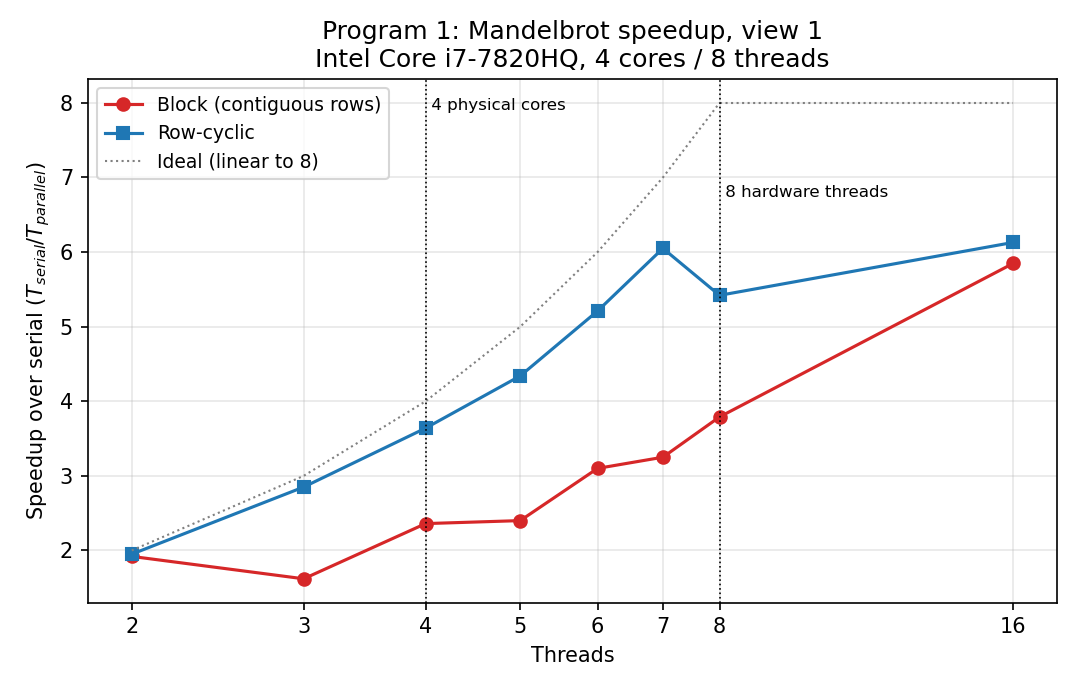
\includegraphics[width=0.85\textwidth]{prog1_speedup_view1.png}
\caption{Speedup versus thread count, view 1. The ideal line is drawn only as
         far as the 8 hardware contexts; beyond that the machine has nothing
         further to give, so the ceiling is flat rather than continuing to
         rise.}
\label{fig:p1v1}
\end{figure}

Speedup under block decomposition is emphatically \textbf{not} linear. Its
efficiency falls from 0.96 at two threads to below 0.60 everywhere
afterwards, and the curve is not even monotonic.

\paragraph{The three-thread datapoint.} Three threads (1.62$\times$) is
\emph{slower} than two (1.92$\times$). Adding a thread made the program worse.

The explanation is the interaction between the cost distribution and the
partition boundaries. Cost per pixel is proportional to iteration count:
pixels inside the set run the full 256 iterations, pixels far outside escape
in two or three, a spread of roughly $100\times$. The set is symmetric about
the real axis, which for view 1 lies at row 600, and its body occupies a dense
band around it.

\begin{itemize}
\item At \textbf{two} threads the split falls at row 600 --- exactly on the
      axis of symmetry. Each thread receives one half of the body. The
      partition is accidentally almost perfect, which is why two threads
      achieves 0.96 efficiency.
\item At \textbf{three} threads the blocks are rows 0--399, 400--799 and
      800--1199. The middle block contains essentially the entire dense band,
      so thread 1 performs most of the work while threads 0 and 2 finish early
      and idle. Speedup collapses.
\item At \textbf{four} threads the body is split between threads 1 and 2, so
      the result recovers somewhat --- but those two threads still carry far
      more work than threads 0 and 3.
\end{itemize}

The hypothesis is therefore that block decomposition distributes \emph{rows}
evenly but \emph{work} very unevenly, and that whether a given thread count
happens to be good or bad depends on where its boundaries fall relative to the
image's axis of symmetry. View 2 (Table~\ref{tab:p1v2}) supports this: it is a
zoomed view with a different cost distribution, and its three-thread point
(2.12$\times$) does not collapse in the same way, because the dense region is
not concentrated into a single block at that thread count.

\subsection{Part 3: per-thread timing confirms the hypothesis}

\texttt{CycleTimer} instrumentation was added at the entry and exit of
\texttt{workerThreadStart()}. It is gated behind the
\texttt{MANDEL\_THREAD\_TIMES} environment variable, because the
\texttt{printf} it performs lies inside the region \texttt{main.cpp} is
timing and would corrupt every other measurement in this report. The
\texttt{getenv} call is evaluated once during static initialisation, before
\texttt{main} runs, so the measured path only reads a boolean.

\begin{table}[H]
\centering
\begin{minipage}{0.47\textwidth}\centering
\progOneBalanceFour
\\[0.4em]{\small Four threads}
\end{minipage}\hfill
\begin{minipage}{0.47\textwidth}\centering
\progOneBalanceEight
\\[0.4em]{\small Eight threads}
\end{minipage}
\caption{Time spent inside \texttt{workerThreadStart()} per thread, view 1,
         from the repetition that set the reported minimum.}
\label{tab:p1balance}
\end{table}

\begin{figure}[H]
\centering
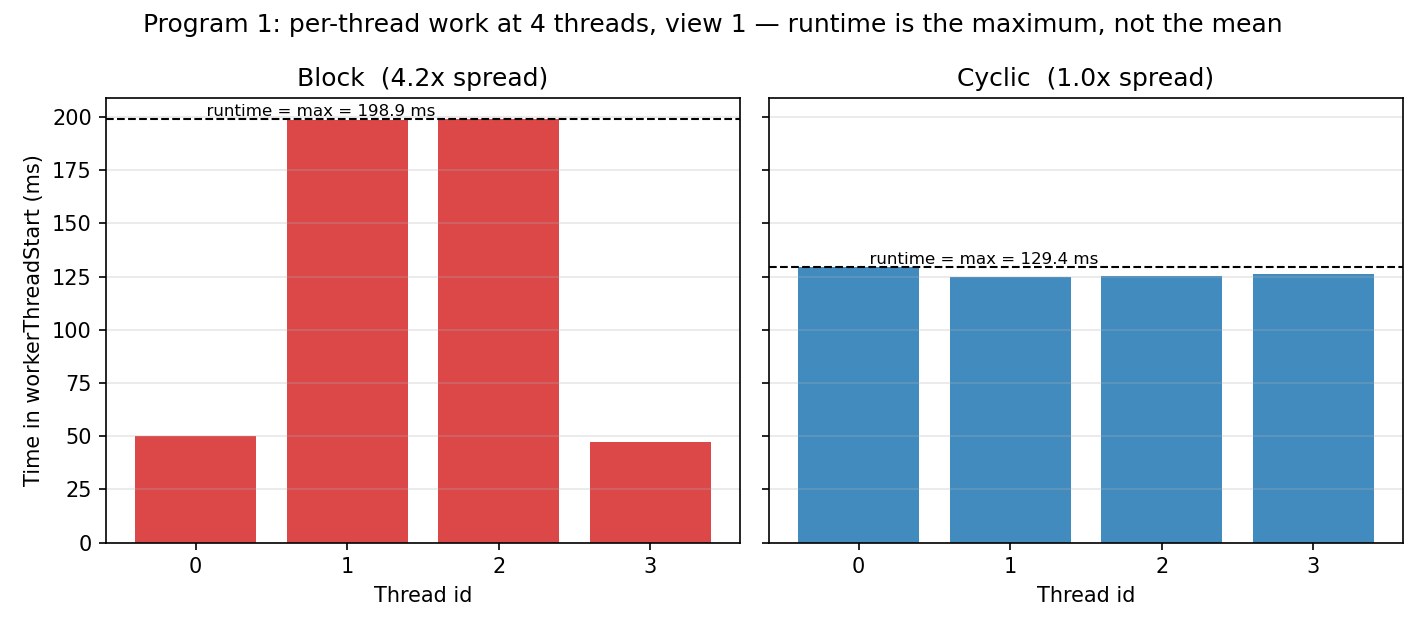
\includegraphics[width=0.92\textwidth]{prog1_threadbalance_t4.png}
\caption{Per-thread work at four threads. Block spreads 4.2$\times$;
         row-cyclic spreads 1.0$\times$.}
\label{fig:p1bal4}
\end{figure}

The measurements confirm the hypothesis exactly. Under block decomposition at
four threads the outer threads take roughly \ms{48} while the inner two take
roughly \ms{199}, a $4.2\times$ imbalance, and the profile has the symmetric
``tent'' shape the cost distribution predicts. At eight threads the spread
widens to $13.3\times$ (\ms{9.3} to \ms{124.4}).

The decisive detail is the total. At eight threads the program reports
\ms{124.331} for the whole image, and thread 3 --- the slowest --- took
\ms{124.4}. \textbf{The runtime of a parallel region is the time of its
slowest thread, not the average of its threads.} Seven threads finishing early
contributes nothing; they simply wait at the join. This is why block
decomposition cannot exceed roughly $3.8\times$ no matter how many threads are
added, and why the speedup curve tracks the maximum per-thread time rather
than the total work divided by $T$.

\subsection{Part 4: row-cyclic decomposition}

The fix follows directly from the diagnosis. The problem is not the amount of
work but its assignment, so the assignment is what changes.

Cost varies \emph{smoothly} with row index --- rows 500 and 508 cost almost
the same --- so giving thread $i$ the rows $i, i+T, i+2T, \dots$ hands every
thread a near-identical sample of the whole cost distribution. Each thread
receives some rows from the dense band and some from the sparse margins, in
the same proportion. No communication, no synchronisation, no dynamic work
queue, and the same rule at every thread count.

The result is immediate. At four threads the per-thread times become
\ms{125.4}, \ms{125.5}, \ms{127.5} and \ms{129.5} --- a spread of
$1.0\times$ against block's $4.2\times$ (Figure~\ref{fig:p1bal4}). The
three-thread point rises from 1.62$\times$ to 2.85$\times$, a $1.76\times$
improvement obtained by executing exactly the same instructions on exactly the
same hardware, changing only which thread runs which row.

Efficiency now stays between 0.83 and 0.97 across the entire range up to eight
threads, rather than collapsing after two.

\textbf{The reported eight-thread speedup is $6.66\times$ on view 1 and
$6.52\times$ on view 2} (minimum of five runs, \texttt{nice -20}; see
Section~\ref{sec:p1sched} for why priority is part of the measurement).

\subsection{The eight-thread anomaly: when the bottleneck is not your code}
\label{sec:p1sched}

At normal priority the row-cyclic results contain something that should not
happen: \textbf{seven threads (6.05$\times$) outperformed eight
(5.42$\times$)}, and sixteen (6.13$\times$) outperformed both.

The per-thread timings showed six threads at \ms{67.2}--\ms{67.7} --- agreeing
to better than 1\% --- and one or two threads at \ms{88}--\ms{100}. Crucially,
\textbf{the slow thread was a different thread in every repetition}: thread 3,
then threads 3 and 7, then 7 and 0, then 0 and 7, then 3 again. The work
assignment is deterministic and byte-identical across repetitions, so a
deterministic decomposition cannot produce a non-deterministic straggler. The
cause had to lie outside the program.

The hypothesis: with eight compute threads on eight hardware contexts there is
no context left over for the kernel, the shell or the display server. Whichever
compute thread the scheduler evicts to run that work loses roughly \ms{30},
and because runtime is the maximum, one eviction costs the entire image.

Two independent measurements were used to test this.

\begin{table}[H]
\centering
\begin{tabular}{r rr}
\toprule
Threads & Involuntary context switches & Runtime (ms) \\
\midrule
4  & 218 & 131.072 \\
7  & 274 & 78.770 \\
8  & \textbf{414} & 82.041 \\
16 & 702 & 73.909 \\
\bottomrule
\end{tabular}
\caption{Involuntary context switches per run, from \texttt{/usr/bin/time -v}.
         The count rises by 51\% moving from seven threads to eight.}
\label{tab:p1cs}
\end{table}

\begin{table}[H]
\centering
\progOnePriority
\caption{View 1, row-cyclic: speedup at normal priority versus
         \texttt{nice -20}. $\star$ marks the only configuration that
         improves.}
\label{tab:p1prio}
\end{table}

Table~\ref{tab:p1prio} is the conclusive result. Raising scheduling priority
improves \textbf{only} the eight-thread configuration, by 22.9\%. Every other
configuration becomes 3--4\% \emph{worse}, because the serial baseline also
runs at elevated priority and drops from \ms{468.5} to \ms{448.6}, reducing
the ratio. That uniform 3--4\% degradation is the control: eight threads
overcomes it and still gains 22.9\%, while four, seven and sixteen threads do
not respond at all.

This is exactly what the hypothesis predicted, including the null results. At
seven threads a context remains free, so there is nothing to preempt and
priority is irrelevant. At sixteen threads oversubscription already absorbs
preemption, so priority is again irrelevant. Only at exactly eight --- full
occupancy with no headroom --- does the effect exist, and removing it recovers
the loss.

With preemption eliminated the curve behaves as the hardware predicts: eight
threads becomes the best configuration at $6.66\times$, and the run-to-run
spread at eight threads falls from 6.6\% to 0.5\%.

\subsection{Part 5: sixteen threads}

\textbf{At normal priority, sixteen threads (6.13$\times$) appeared faster than
eight (5.42$\times$). Under controlled conditions the ordering reverses:
sixteen threads (6.33$\times$) is 5\% \emph{slower} than eight
(6.66$\times$).}

Performance is therefore not meaningfully greater at sixteen threads, and the
apparent gain at normal priority was an artefact.

The reason is that the processor provides only eight hardware contexts. Beyond
that, additional threads do not execute concurrently --- they time-share
contexts that are already saturated, adding context-switch overhead and
scheduling jitter while contributing no additional parallelism. The 8.8\%
run-to-run spread at sixteen threads, against 0.5\% at eight, is that jitter
made visible.

The apparent advantage at normal priority was not a benefit of
oversubscription but a \emph{workaround} for the preemption problem of
Section~\ref{sec:p1sched}: with two threads per context each holding half the
work, an eviction costs half as much and the scheduler can interleave around
it. Once the underlying problem was removed, the workaround became pure
overhead. That the sixteen-thread figure at normal priority (6.13$\times$) sits
so close to the seven-thread figure (6.05$\times$) is the same fact from
another angle --- both are ways of leaving the scheduler room, and neither
exceeds what eight unimpeded threads achieve.

\subsection{Achieved speedup against the machine's ceiling}
\label{sec:p1target}

\begin{table}[H]
\centering
\begin{tabular}{lrr}
\toprule
Configuration & Mean clock (MHz) & Peak clock (MHz) \\
\midrule
1 thread  & 3110 & 3881 \\
2 threads & 3093 & 3886 \\
4 threads & 3062 & 3908 \\
8 threads & 2992 & \textbf{3704} \\
\bottomrule
\end{tabular}
\caption{Core clock sampled during execution, \texttt{performance} governor.}
\label{tab:p1clock}
\end{table}

The achieved figure is $6.66\times$ at eight threads, against the handout's
stated target of roughly $7$--$8\times$. Three measured effects account for the
difference.

\textbf{Scaling across physical cores is near-ideal.} Four threads reach
$3.61\times$, an efficiency of 0.902. The decomposition is not the limiting
factor; at four threads the per-thread spread is $1.0\times$.

\textbf{Hyper-Threading contributes $1.845\times$ on top of four cores}
($6.66 / 3.61$). This is unusually high --- typical SMT gains are 1.2--1.3$\times$
--- and it is a property of this workload. The inner loop of \texttt{mandel()}
is a serial dependency chain of floating-point multiplies and adds in which
each iteration's \texttt{z\_re} depends on the previous iteration's. It is
latency-bound with low instruction-level parallelism, leaving pipeline slots
empty that a second thread on the same core can fill almost for free.
Mandelbrot is close to a best case for SMT, and Program~5 will show the
opposite extreme.

\textbf{Turbo headroom is lost at full occupancy.} Table~\ref{tab:p1clock}
shows peak clock holding at 3881--3908\,MHz up to four threads and falling to
3704\,MHz at eight, a drop of 4.6\%. The serial baseline is therefore timed at
a clock the eight-thread run cannot sustain, so part of the ``missing''
speedup was never physically available. Normalising for it gives
$6.66 \times (3881/3704) = 6.98\times$, i.e.\ essentially $7\times$ in
clock-equivalent terms.

This is the expected difference between this machine and the \texttt{myth}
reference. The i7-7700K is a 91\,W desktop part whose all-core turbo (4.4\,GHz)
sits within 2\% of its single-core turbo (4.5\,GHz); the i7-7820HQ is a 45\,W
mobile part in a laptop chassis, where sustaining all eight contexts costs
measurable clock. The gap between $6.66\times$ and the quoted target is
accounted for by that, not by the decomposition.

\subsection{Summary}

\begin{table}[H]
\centering
\begin{tabular}{lll}
\toprule
Part & Result & Key observation \\
\midrule
1--2 & Block: 1.92$\times$ at 2, \textbf{1.62$\times$ at 3} & Three threads is slower
       than two; boundaries \\
     & & land relative to the axis of symmetry \\
3    & Spread 4.2$\times$ at 4, 13.3$\times$ at 8 & Runtime equals the slowest thread,
       not the mean \\
4    & Row-cyclic: \textbf{6.66$\times$ at 8 threads} & Spread falls to 1.0$\times$;
       three-thread point \\
     & & improves 1.76$\times$ from remapping alone \\
5    & 16 threads: 6.33$\times$, 5\% slower than 8 & Only 8 hardware contexts exist \\
\bottomrule
\end{tabular}
\end{table}

\paragraph{What this program demonstrates.} The runtime of a parallel region is
set by its slowest participant, so load balance --- a question of
\emph{mapping}, not of code optimisation --- dominates. A static interleaving
achieved this with no synchronisation whatsoever, because the cost function
varies smoothly across the domain. And when measurements became
non-deterministic while the program remained deterministic, the cause was
necessarily outside the program: the eight-thread deficit was a scheduling
artefact of running exactly as many compute threads as the machine has
contexts, not a property of the algorithm.

%======================================================================
\section{Program 2: Vectorizing Code Using SIMD Intrinsics}
%======================================================================

\subsection{What is being measured}

This program uses the CS149 ``fake'' vector intrinsics, which simulate a SIMD
unit rather than compiling to real AVX2 instructions. Consequently
\emph{nothing in this section is a timing}. ``Total Vector Instructions'' and
``Vector Utilization'' are exact counts of simulated operations: they are
bit-for-bit reproducible, independent of machine load, and identical on every
run. The five-run minimum protocol of Section~2 therefore does not apply here,
and a single run per width is exhaustive rather than merely adequate. Following
the handout, one fake vector instruction is treated as costing one cycle, so
instruction count is the performance measure.

Note also that \texttt{printStats()} is invoked before \texttt{arraySumVector()}
is called, so every figure below describes \texttt{clampedExpVector()} alone.

\subsection{Implementation}

The serial function raises \texttt{values[i]} to the power
\texttt{exponents[i]} by repeated multiplication and clamps the result at
$9.999999$. Three aspects required care.

\paragraph{Divergent trip counts.} Each lane needs a different number of
multiplications. A vector unit cannot let one lane exit a loop early, so the
loop runs until the \emph{slowest} lane in the vector is finished, with
completed lanes masked off. The mask \texttt{maskActive} is recomputed from
\texttt{count > 0} after every iteration and the loop continues while
\texttt{\_cs149\_cntbits(maskActive) > 0}.

\paragraph{The \texttt{y == 0} special case needs no branch.} The serial code
treats a zero exponent separately, returning $1.f$. Initialising
\texttt{result} to $1.f$ and multiplying $y$ times produces $x^y$ for $y > 0$
and leaves $1.f$ untouched for $y = 0$, since such a lane is never active. This
removes a branch that would otherwise have cost an extra mask and a masked
store. The subsequent clamp is likewise applied unconditionally to all active
lanes: a $y = 0$ lane holds $1.f$, which is below the ceiling, so the result is
unaffected.

\paragraph{Partial final vector.} When \texttt{VECTOR\_WIDTH} does not divide
$N$, the last iteration covers fewer than \texttt{VECTOR\_WIDTH} elements.
Enabling only the valid lanes, by passing
$\min(\texttt{VECTOR\_WIDTH},\, N-i)$ to \texttt{\_cs149\_init\_ones}, keeps
the store from writing past $N$ --- \texttt{main.cpp} checks for exactly this and reports
\emph{``You have written to out of bound value''} --- and keeps the dead lanes
out of the utilization statistics.

This is the flaw in the supplied \texttt{absVector()} example, which the
handout invites the reader to find: its loop advances by
\texttt{VECTOR\_WIDTH} under an unconditional all-ones mask, so for
$N \bmod \texttt{VECTOR\_WIDTH} \neq 0$ it reads and writes past the end of the
arrays.

One further initialisation detail matters. \texttt{\_cs149\_vgt\_int} leaves
masked-off lanes at their previous value, so \texttt{maskActive} is explicitly
cleared with \texttt{\_cs149\_init\_ones(0)} before first use. Without this,
lanes beyond the array end would inherit stale values and could appear active.

The implementation was verified across 32 configurations --- widths
$\{2,4,8,16\}$ against $N \in \{1,2,3,5,7,15,17,100\}$ --- all of which produce
correct results with no out-of-bounds write.

\subsection{Width sweep}

\begin{table}[H]
\centering
\small
\progTwoWidths
\caption{$N = 10000$. ``Inner-loop utilization'' is measured separately, as
         described in Section~5.4. At this $N$ every width divides evenly
         ($10000/16 = 625$), so no partial vector occurs and the trend is
         entirely attributable to divergence.}
\label{tab:p2widths}
\end{table}

\begin{figure}[H]
\centering
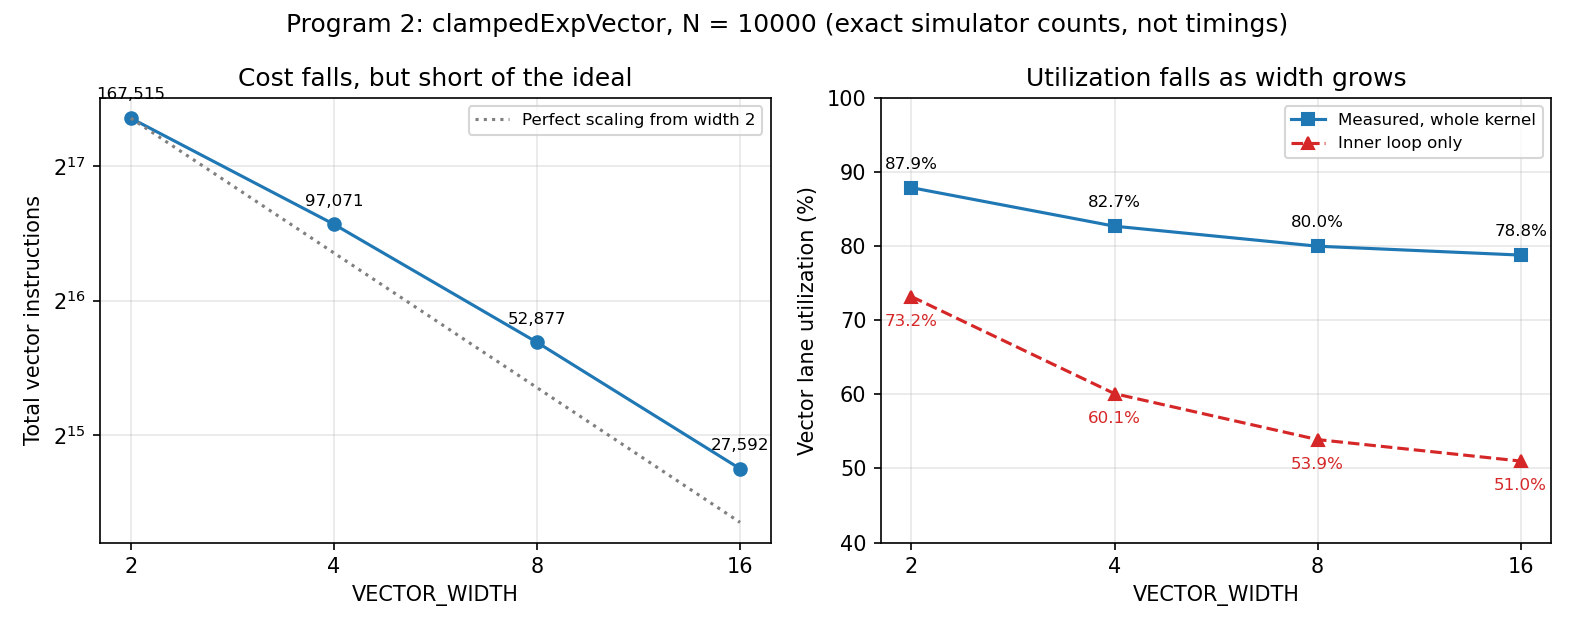
\includegraphics[width=\textwidth]{prog2_width_sweep.png}
\caption{Instruction count and lane utilization against vector width.}
\label{fig:p2}
\end{figure}

\textbf{Vector utilization decreases monotonically as
\texttt{VECTOR\_WIDTH} increases}: 87.9\%, 82.7\%, 80.0\%, 78.8\%.

\subsection{Why utilization falls}

The cause is \emph{divergence}. The exponents are drawn uniformly from
$[0, 9]$, so lanes within a vector need different numbers of multiplications,
and the vector must keep iterating until its slowest lane finishes. Every
iteration a lane spends already finished is an enabled slot doing no useful
work.

The wider the vector, the more lanes must agree for the loop to stop early ---
and the more likely it becomes that at least one lane drew a large exponent.
With two lanes the expected maximum exponent is well below $9$; with sixteen it
is close to $9$ almost every time, so nearly every vector runs the full nine
iterations regardless of what the other fifteen lanes needed.

To measure this rather than assert it, \texttt{analyze\_divergence.cpp}
reproduces the exact exponent array \texttt{main.cpp} generates (same
\texttt{rand()} sequence, same \texttt{EXP\_MAX}) and counts how much of the
inner loop's lane capacity is useful.

\begin{table}[H]
\centering
\progTwoDivergence
\caption{Inner-loop divergence at $N = 10000$. The work actually required is
         fixed at 44\,835 multiplications regardless of width; the lane
         capacity consumed to deliver it grows by 43\%.}
\label{tab:p2div}
\end{table}

The work required never changes --- 44\,835 multiplications --- yet the lane
capacity spent on it rises from 61\,256 at width 2 to 87\,856 at width 16.
Inner-loop utilization accordingly falls from 73.2\% to 51.0\%: \textbf{at
width 16 roughly half of all enabled lane-slots in the loop are doing nothing}.

The measured whole-kernel figure (78.8\% at width 16) is higher than the
loop-only figure (51.0\%) because the surrounding instructions --- the two
loads, the store, the initial \texttt{vset}, \texttt{vmove}, and the clamp ---
run with every lane enabled and never diverge. They dilute the divergence
penalty, which is why the measured curve declines more gently than the
underlying mechanism does.

\subsection{Cost, and why wider still wins}

Falling utilization does not mean wider vectors are worse. Total instruction
count drops from 167\,515 to 27\,592, a $6.07\times$ reduction for an
$8\times$ increase in width. Utilization measures \emph{efficiency}; instruction
count measures \emph{cost}. Efficiency falls while cost falls faster.

The marginal returns are the interesting part. Successive doublings of width
reduce instruction count by $1.73\times$, $1.84\times$ and $1.92\times$ --- the
benefit \emph{improves} as vectors widen, approaching the ideal $2\times$.

Two opposing effects explain this. Per-vector fixed overhead (loads, store,
masks, clamp --- roughly a dozen instructions independent of exponent values)
is amortised over twice as many elements at each doubling, which always helps.
Against that, divergence costs more as width grows --- but only up to a point,
because the exponent range is bounded at $9$. Once vectors are wide enough that
almost every one contains a near-maximal exponent, widening further adds
essentially no extra iterations while still halving the number of vectors. The
divergence penalty saturates; the amortisation does not. The loop-iteration
counts show the same saturation directly: $30\,628 \to 18\,642 \to 10\,406 \to
5\,491$, ratios of $1.64$, $1.79$, $1.90$, converging on $2$.

\subsection{Extra credit: vectorized array sum}

\texttt{arraySumVector()} replaces $N$ scalar additions with two phases.

\textbf{Phase 1} folds the array into a single register with $N/W$ vector
additions, leaving $W$ partial sums, one per lane. \textbf{Phase 2} reduces
those $W$ lanes to one value in $\log_2 W$ rounds of
\texttt{hadd} followed by \texttt{interleave}. \texttt{hadd} sums adjacent
pairs and duplicates each result across the pair; \texttt{interleave} then
moves even-indexed lanes into the front half, packing the distinct partial sums
adjacent to one another so the next \texttt{hadd} pairs them. After $\log_2 W$
rounds every lane holds the total.

For $W = 4$ and lanes $[a\;b\;c\;d]$:
\[
[a\;b\;c\;d]
\xrightarrow{\text{hadd}} [a{+}b\;\;a{+}b\;\;c{+}d\;\;c{+}d]
\xrightarrow{\text{interleave}} [a{+}b\;\;c{+}d\;\;a{+}b\;\;c{+}d]
\xrightarrow{\text{hadd}} [T\;T\;T\;T]
\]
where $T = a+b+c+d$. Total cost is $N/W + 2\log_2 W$ vector operations against
$N$ scalar additions, meeting the $O(N/W + \log_2 W)$ target. The
implementation passes for every width tested.

\subsection{Summary}

\begin{table}[H]
\centering
\begin{tabular}{ll}
\toprule
Question & Answer \\
\midrule
Does utilization change with width? & It \textbf{decreases}: 87.9\% $\to$ 78.8\% \\
Why? & Divergence. Lanes need different trip counts, and \\
     & the vector runs until its slowest lane finishes. \\
Measured mechanism & Inner-loop utilization falls 73.2\% $\to$ 51.0\% \\
Is wider still better? & Yes --- cost falls $6.07\times$ while efficiency falls \\
\bottomrule
\end{tabular}
\end{table}

\paragraph{What this program demonstrates.} SIMD efficiency is governed by how
uniform the work is across lanes, not by how much work there is. The same total
computation --- a fixed 44\,835 multiplications --- costs progressively more
lane capacity as vectors widen, purely because the lanes disagree about when to
stop. Utilization and cost are distinct measures that can and do move in
opposite directions: a kernel can become less efficient and faster at the same
time. And divergence penalties are bounded by the spread of the work, not by
the width, which is why the marginal return to widening improves rather than
degrades once the spread is saturated.

\end{document}
